\documentclass[a4paper]{llncs}
\usepackage[utf8]{inputenc}
\usepackage{amsmath,amssymb}
\usepackage{tikz}
\usepackage{hyperref}
\usepackage{wrapfig}

\newcommand{\defo}[1]{\emph{#1}}

\renewcommand{\sectionautorefname}{Section} 

\newcommand{\abovebelow}[2]{(^{#1}_{#2})}

\newcommand{\rank}{r}
\newcommand{\inv}{s}
\newcommand{\ranki}{\mathring{r}}
\newcommand{\invi}{\mathring{s}}
\newcommand{\tr}[1]{{#1}\!\strut^\intercal\!}
\newcommand{\BMS}{\text{\tiny\textsc{BMS}}}

\definecolor{rkBlue}{RGB}{50,20,230}
\definecolor{siGreen}{RGB}{0,103,0}



\title{Linear Ranking for Linear Lasso Programs\thanks{
The final publication is available at \href{http://link.springer.com/chapter/10.1007\%2F978-3-319-02444-8_26}{link.springer.com}.
} \thanks{
  This work is supported by the
  German Research Council (DFG) as part of the Transregional Collaborative
  Research Center ``Automatic Verification and Analysis of Complex Systems''
  (SFB/TR14 AVACS)
}
}

\author{Matthias Heizmann \and Jochen Hoenicke\and Jan Leike \and Andreas Podelski}

\institute{University of Freiburg, Germany}



\begin{document}

\maketitle              


\sloppy

\begin{abstract}
The general setting of this work is the constraint-based synthesis of termination arguments.
We consider a restricted class of programs called lasso programs. The termination argument for a lasso program is a pair of a ranking function and an invariant.
We present the---to the best of our knowledge---first method to synthesize termination arguments for lasso programs that uses  linear arithmetic.
We prove a completeness theorem.
The completeness theorem establishes that, even though we use only linear (as opposed to non-linear) constraint solving, we are able to compute termination arguments in several interesting cases.
The key to our method lies in a constraint transformation that replaces a disjunction by a sum.
\end{abstract}



\section{Introduction}
Termination is arguably the single most interesting correctness property of a program.
Research on proving termination can be divided according to three (interrelated) topics, namely:
practical tools~\cite{DBLP:journals/jar/AlbertAGP11,cav/BrockschmidtMOG12,cav/CookPR06,sas/HarrisLNR10,atva/KroeningSTTW08,cav/KroeningSTW10,lics/PodelskiR04,hybrid/PodelskiW07},
\mbox{decidability} questions~\cite{vmcai/Ben-AmramGM12,cav/Braverman06,cav/Tiwari04}, 
and
constraint-based synthesis of
termination \mbox{arguments}
~\cite{DBLP:journals/iandc/BagnaraMPZ12,DBLP:journals/corr/abs-1208-4041,cav/BradleyMS05,icalp/BradleyMS05,concur/BradleyMS05,tacas/ColonS01,journals/fmsd/CookKRW13,vmcai/Cousot05,vmcai/PodelskiR04,cav/Rybalchenko10}.  The work in this paper falls under the research on the third topic.
The general goal of this research is to investigate how one can derive a constraint from the program text and compute a termination argument (of a restricted form) through the solution of the constraint, i.e., via constraint solving.

In this paper, we present a method for the synthesis of termination arguments for a specific class of programs that we call \emph{lasso programs}. 
As the name indicates, the control flow graph of a lasso program is of a restricted shape: a \emph{stem} followed by a \emph{loop}.

Lasso programs do not appear as stand-alone programs.
Lasso programs appear in practice whenever one needs a finite representation of an infinite path in a control flow graph, for example in (potentially spurious) counterexamples in a termination analysis\cite{cav/CookPR06,sas/HarrisLNR10,atva/KroeningSTTW08,cav/KroeningSTW10},  non-termination analysis\cite{conf/popl/GuptaHMRX08}, stability analysis\cite{vmcai/CookFKP11,hybrid/PodelskiW07}, or cost analysis\cite{DBLP:journals/jar/AlbertAGP11,conf/pldi/GulwaniZ10}.

Importantly, the termination argument for a lasso program is a pair of a ranking function and an invariant (the rank must decrease only for states that satisfy the invariant). \autoref{fig-bangalore} shows an example of a lasso program.

The class of lasso programs lies between two classes of programs for which constraint-based methods have been studied extensively. 
For the first, more specialized class, methods can be based on linear arithmetic constraint solving~\cite{DBLP:journals/iandc/BagnaraMPZ12,DBLP:journals/corr/abs-1208-4041,tacas/ColonS01,journals/fmsd/CookKRW13,vmcai/PodelskiR04}. 
For the second, more general class, all known methods are based on non-linear arithmetic constraint solving~\cite{cav/BradleyMS05,concur/BradleyMS05}. 
The contribution of our method can be phrased, alternatively, as the generalization of the applicability of the `linear methods', or as the
optimization of the `non-linear method' to a `linear method' for a subproblem.
The step from `non-linear' to `linear' is interesting for principled reasons (non-linear arithmetic constraint solving is undecidable in the case of integers).
As we will show the step is also practically interesting.

The reader may wonder how practical tools presently handle the situation where one needs to compute  termination arguments for lasso programs. 
One possibility is to resort to heuristics.
  For example, instead of computing a termination argument for the lasso program in Figure 1, one would compute the ranking function  for the program \verb|while(x>=0){x:=x-23;}|.

The key to our method is a constraint transformation that replaces a disjunction by a sum. We apply the `or-to-plus' transformation in the context of Farkas' Lemma.  
Following~\cite{DBLP:journals/iandc/BagnaraMPZ12,cav/BradleyMS05,tacas/ColonS01,journals/fmsd/CookKRW13,vmcai/PodelskiR04}, we apply Farkas' Lemma in order to eliminate the universal quantifiers in the arithmetic constraint whose solution is the termination argument.
If we apply Farkas' Lemma to the constraint \emph{after} the `or-to-plus' transformation, we obtain a \emph{linear} arithmetic constraint.

The effect of the `or-to-plus' transformation to the constraint is a restriction of its solution space.  The restriction seems strong; i.e., in some cases, the solution space becomes empty.
We can characterize those cases. In other words, we can characterize when the `or-to-plus' transformation leads to the loss of an termination argument, and when it does not.
The characterization is formulated as a completeness theorem for which we will present the proof.
This characterization allows us to establish that, even though we use only linear (as opposed to non-linear) constraint solving, we are able to compute termination arguments in several interesting cases.
A possible explanation for this (perhaps initially surprising) fact is that, for synthesis, we are interested in the mere existence of a solution, and the loss of \emph{many} solutions does not necessarily mean the loss of \emph{all} solutions of the constraint.  


\begin{figure}[t]
\begin{center}
\begin{minipage}{4cm}

\begin{verbatim}
1: y := 23;
2: while( x >= 0 ) {
3:     x := x - y;
4:     y := y + 1;
5: }
\end{verbatim}

\end{minipage}
\begin{minipage}{6cm}
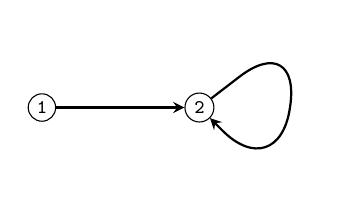
\begin{tikzpicture}[auto,
trans/.style={->,>=stealth,thick}]
 \node (0) at (0,0) [circle,draw,inner sep=1.5] {\scriptsize \texttt{1}};
 \node (1) at (2,0) [circle,draw,inner sep=1.7] {\scriptsize \texttt{2}};
\draw [trans] (0) to node[] {} (1);
\draw [trans,rounded corners=10mm, pos=0.1] (1) -- (3.3,1) -- node {} (3,-1) --  (1);

\end{tikzpicture}
\end{minipage}
\end{center}
\caption{Example of a lasso program and its formal representation .
The ranking function defined by  decreases in transitions from states that satisfy the invariant  (the ranking function does not decrease when ).
}
\label{fig-bangalore}
\end{figure}


We have implemented our method and we have used our implementation to illustrate the applicability and the efficiency of our method. Our implementation is available through a web interface, together with a number of example programs (including the ones used in this paper).\footnote{
\url{http://ultimate.informatik.uni-freiburg.de/LassoRanker}
}


\section{Preliminaries: Linear Arithmetic}
We use  to denote the vector with entries , and  to denote the transposed vector of .
As usual, the expression  denotes the conjunction of linear constraints .

We call a relation  a \defo{linear relation} if  is defined by a conjunction of linear constraints over the variables  and , i.e., if there is a matrix  with  rows and  columns and a vector  of size  such that the following equation holds.


We call a function  an \defo{(affine) linear function}, if  is defined by an affine linear term, i.e., there is a vector  and a number  such that the following equation holds.


We call a predicate  a \defo{linear predicate}, if  is defined by a linear inequality, i.e., there is a vector  and a number  such that following equivalence holds.



\paragraph{Farkas' Lemma.} We use the affine version of Farkas' Lemma~\cite{Schrijver:1986:TLI:17634} which is also used in ~\cite{DBLP:journals/iandc/BagnaraMPZ12,cav/BradleyMS05,journals/fmsd/CookKRW13,cav/Rybalchenko10,vmcai/PodelskiR04} and states the following.
Given
\begin{itemize}
 \item a satisfiable conjunction of linear constraints 
 \item and a linear constraint ,
\end{itemize}
the following equivalence holds.
\begin{center}
 \ \ \ iff \ \ \  
\end{center}












\section{Lasso Program}
To abstract away from program syntax, we define a lasso program directly by the two relations that generate its execution sequences.

\begin{definition}[Lasso Program] Given a set of states , a \defo{lasso program} 

is given by the two relations  and .
We call  the \defo{stem} of  and  the \defo{loop} of .

An \defo{execution of the lasso program}  is a possibly infinite sequence of states  such that
\begin{itemize}
 \item the pair of the first two states is an element of the stem, i.e.,
 
 \item and each other consecutive pair of states is an element of the loop, i.e.,
 
\end{itemize}
We call the lasso program  \defo{terminating} if  has no infinite execution.

\end{definition}
We use constraints over primed and unprimed variables to denote a transition relation (see~\autoref{fig-bangalore}).


In order to avoid cumbersome technicalities, we consider only lasso programs that have an execution that contains at least three states. This means we consider only programs where the relational composition of  and  is non-empty, i.e.,




Since Turing, a termination argument is based on an ordering which does not allow infinite decreasing chains (such as ordering on the natural numbers).  Here, we use the ordering over the set of positive reals which is defined by some value , namely

\begin{center}
\hfil\hfil\hfil  \ \ \ \  iff \ \ \ \   \hfil\hfil\hfil  
\end{center}

\paragraph{Ranking Function.}
We call a function  from the states of the lasso program  into
the reals  a \defo{ranking function} for  if there is a
positive number  such that for each consecutive pair of
states  of a loop transition ()
in every execution of 
\begin{itemize}
\item the value of  is decreasing by at least , i.e.,

\item and the value of  is non-negative, i.e.,

\end{itemize}
If there is a ranking function for the lasso program , then  is terminating.


\paragraph{Inductive Invariant.}
We call a state predicate  an \defo{inductive invariant} of the lasso program  if

\begin{itemize}
\item the predicate holds after executing the stem, i.e.,



\item and if the predicate holds before executing the loop, then the predicate holds afterwards, i.e.,

\end{itemize}



\paragraph{Ranking Function with Supporting Invariant.}
We call a pair of a ranking function  and an inductive invariant  of the lasso program  a \emph{ranking function with supporting invariant} if the following holds.
\begin{itemize}
\item There exists a positive real number  such that, if the inductive invariant holds then an execution of the loop decreases the value of the ranking function by at least , i.e.,

\item In states in which the inductive invariant holds and the loop can be executed, the value of the ranking function is non-negative, i.e., 

\end{itemize}

For example, the lasso program depicted in \autoref{fig-bangalore} has the ranking function   with supporting invariant .

\paragraph{Linear lasso programs.}
Linear lasso programs. For the remainder of this paper we consider only linear lasso programs, linear ranking functions, and linear inductive invariants which we will define next.  The variables of the programs will range over the reals until we come to Section 9 where we turn to programs over integers.


\begin{definition}[Linear Lasso Program]
A \defo{linear lasso program}  is a lasso program whose states are vectors over the reals, i.e. , and whose relations  and  are linear relations.
\end{definition}
We use the expression  to denote the relation  of .
We use the expression  to denote the relation  of .

\paragraph{Linear Ranking Function.}
If a ranking function  is an (affine) linear function, we call  a \defo{linear ranking function}.
We use  as coefficients of a linear ranking function,  as their vector,



\paragraph{Linear Invariant.}
If an inductive invariant  is a linear predicate, we call  a \defo{linear inductive invariant}. 
We use  as coefficients of the term that defines the linear predicate,  as their vector,










\section[The Or-to-Plus Method]{The Or-to-Plus Method}

Our constraint-based method for the synthesis of linear ranking functions for linear lasso programs consists of three main steps:
\begin{description}
 \item[Step 1.] Set up four (universally quantified) constraints whose free variables are the coefficients of a linear ranking function with linear supporting invariant.
 \item[Step 2.] Apply Farkas' Lemma to the four constraints to obtain equivalent constraints without universal quantification.
 \item[Step 3.] Obtain solutions for the free variables by linear constraint solving.
\end{description}

The particularity of  our four constraints in Step~1
is that the application of Farkas' Lemma in Step~2 yields constraints that are linear.

Instead of presenting our constraints immediately, we derive them in three successive transformations of constraints.
We start with the four constraints \eqref{inv-stem1}, \eqref{inv-loop1}, \eqref{rk-decr1}, and \eqref{rk-bound1}.
Below, we have rephrased the four constraints for the setting where the ranking function is linear and the supporting invariant is linear.
We marked them \eqref{inv-stem2}, \eqref{inv-loop2}, \eqref{rk-decr2}, and \eqref{rk-bound2} in reference to Bradley, Manna and Sipma [5] who were the first to use them in the corresponding step of their method.



\subsubsection{The Bradley--Manna--Sipma constraints}\noindent

\noindent{\scriptsize for the special case of lasso programs and one linear supporting invariant}\footnote{
In~\cite{cav/BradleyMS05} the authors use more general general constraints that can be used to synthesize lexicographic linear ranking functions together with a conjunction of linear supporting invariants for programs that can also contains disjunctions.}

The free variables of
 are , , , and .






\subsubsection{Transformation 1: Move supporting invariant to right-hand side.}
We bring the conjunct
 
in three of the four constraints \eqref{inv-stem2}, \eqref{inv-loop2}, \eqref{rk-decr2}, and \eqref{rk-bound2}
to the right-hand side of the implication, according to the following scheme.

We obtain the following constraints.




\subsubsection{Transformation 2: Drop supporting invariant in fourth constraint.}
We strengthen the fourth constraint \eqref{rk-bound3} by removing the disjunct .
A solution for the strengthened constraint defines a ranking function
whose value is bounded from below for all states (and not just those that
satisfy the supporting invariant).

\subsubsection[Step 3: Replace disjunction by sum.]{Transformation 3: Replace disjunction by sum.}
We replace the disjunction on the right-hand side of the implication in constraints \eqref{inv-loop3} and \eqref{rk-decr3} by a single inequality, according to the scheme below. (It is the disjunction which prevents us from applying Farkas' Lemma to the constraints \eqref{inv-loop3} and \eqref{rk-decr3}.)

In the second constraint~\eqref{inv-loop3}, we replace the disjunction 

by the inequality 

In the third constraint~\eqref{rk-decr3}, we replace the disjunction 

by the inequality

We obtain the following four constraints.
\subsubsection{The Or-to-Plus constraints}\noindent

The free variables of the conjunction  are , , , and .
\bigskip


Since we consider linear lasso programs, the relations  and  are given as conjunctions of linear constraints.


\bigskip



We have now finished the description for the three transformation steps that lead us to the the or-to-plus constraints. We are now ready to introduce our method.

\medskip

\begin{center}
\fbox{
 \begin{minipage}{11cm}
 \textbf{The Or-to-Plus Method}

  \begin{description}
  \item[Input:] linear lasso program .
  \item[Output:] coefficients , , , and  of a linear ranking function with linear supporting invariant
 \end{description}

 
  
 \begin{enumerate}
  \item Set up the or-to-Plus constraints \ref{inv-stem4},  \ref{inv-loop4}, \ref{rk-decr4}, and \ref{rk-bound4} for .
  \item Apply Farkas' Lemma to each constraint.
  \item Obtain , , , and ,  by linear constraint solving.
 \end{enumerate}
 \end{minipage}
}
\end{center}

\medskip

After setting up the four or-to-plus constraints , , ,  in Step~1, we apply Farkas' Lemma to each of the four constraints in Step~2.
We obtain four linear constraints.
E.g., by applying Farkas' Lemma to the constraint~\eqref{rk-decr4} we obtain the following linear constraint.



We apply linear constraint solving in Step~3. We obtain a satisfying assignment for the free variables in the resulting constraints.
The values obtained for , ,  and   are the coefficients of a linear ranking function  with linear supporting invariant .



The or-to-plus method inherits its soundness from method of Bradley--Manna--Sipma. 
Step~1 is an equivalence
transformation on the Bradley--Manna--Sipma constraints, Step~2 and
Step~3 strengthen the constraints, and the application of Farkas' Lemma
is an equivalence transformation.   Thus, a satisfying assignment of the
or-to-plus constraints obtained after the application of Farkas' Lemma is also a satisfying assignment of the Bradley--Manna--Sipma constraints.









\section{Completeness of the Or-to-Plus Method}

In the tradition of constraint-based synthesis for verification, we
will formulate completeness according to the following scheme: the method
\texttt{X} applied to a program  in the class \texttt{Y} computes (the
coefficients of) a correctness argument of the form \texttt{Z}
whenever one exists (i.e., whenever a correctness argument of the form
\texttt{Z} exists for the program ).  Here, \texttt{X} is the
or-to-plus method, \texttt{Y} is the class of lasso programs, and
\texttt{Z} is a termination argument consisting of a linear ranking
function and an invariant of a form that we we define next.

\begin{definition}[Non-decreasing linear inductive invariant]
We call a linear inductive invariant  of the lasso program P \emph{non-decreasing} if the loop implies that the value of the term  does not decrease when executing the loop, i.e.,

\end{definition}

In \autoref{sec:examples} we give examples which may help to convey some
intuition about the meaning of `non-decreasing', examples of those
terminating programs that do have a linear ranking function with a
non-decreasing linear supporting invariant, and examples of those that
don't.  

\begin{figure}[t]
\begin{center}
\begin{minipage}{4cm}
\begin{verbatim}
x := y + 42;
while( x >= 0 ) {
    y := 2*y - x;
    x := (y + x) / 2;
}
\end{verbatim}

\end{minipage}
\begin{minipage}{6cm}
\vspace{-8mm}
2mm]
 \tau_\mathsf{loop}: & x\geq 0 \;\land\; x'=y \;\land\; y'=2y-x
\end{array}
\forall\vec x\quad A\cdot  \vec x \leq \vec b \;\rightarrow\; \tr{\vec g}\cdot  \vec x + g_0\geq 0 \;\lor\; \tr{\vec h}\cdot  \vec x + h_0> 0,\forall\vec x\quad A\cdot  \vec x \leq \vec b \;\rightarrow\;
(\tr{\vec g}\cdot \vec x + g_0) + \mu \cdot (\tr{\vec h}\cdot \vec x + h_0)\geq 0.
\forall\vec x \quad A\cdot\vec x \leq \vec b \;\rightarrow\; (\tr{\vec g}
\cdot\vec x + g_0 \geq 0 \;\lor\; \tr{\vec h}\cdot\vec x + h_0 > 0)

\forall\vec x \quad (A\cdot\vec x \leq \vec b
\;\land\; \tr{\vec h}\cdot\vec x + h_0 \leq 0) \;\rightarrow\; \tr{\vec g}
\cdot\vec x + g_0 \geq 0.

\exists \mu \geq 0 \;\exists \vec\lambda \geq 0
\quad \mu \cdot \tr{\vec h} + \tr{\vec\lambda}\cdot A = -\tr{\vec g}
\;\land\; \tr{\vec\lambda}\cdot\vec b + \mu \cdot (-h_0) \leq g_0,

\exists \mu \geq 0 \;\exists \vec\lambda \geq 0
\quad \tr{\vec\lambda}\cdot A = -(\mu \cdot \tr{\vec h} + \tr{\vec g})
\;\land\; \tr{\vec\lambda}\cdot\vec b \leq \mu \cdot h_0 + g_0.
\exists \mu \geq 0 \;\forall\vec x \qquad A\cdot\vec x \leq \vec b
\;\rightarrow\; -(\mu \cdot \tr{\vec h} + \tr{\vec g})\vec x \leq \mu
\cdot h_0 + g_0. \quad\qed
A_\mathsf{loop}\cdot(^{\vec x}_{\vec x'})\leq \vec b_\mathsf{loop}
\;\rightarrow\; -\tr{\vec{\invi}}\cdot \vec x - \invi_0 > 0
\label{eq-completeness-executable}
\tr{\vec{\invi}}\cdot \vec x + \invi_0\geq 0 \;\land\;
A_\mathsf{loop}\cdot(^{\vec x}_{\vec x'})\leq \vec b_\mathsf{loop}
\;\rightarrow\;  \tr{\vec{\ranki}}\cdot \vec x+\ranki_0 \geq 0,A_\mathsf{loop}\cdot(^{\vec x}_{\vec x'})\leq \vec b_\mathsf{loop}
\;\rightarrow\;  \tr{\vec{\ranki}}\cdot \vec x+\ranki_0\geq 0 \;\lor\;
-\tr{\vec{\invi}}\cdot \vec x - \invi_0 > 0A_\mathsf{loop}\cdot(^{\vec x}_{\vec x'})\leq \vec b_\mathsf{loop}
\;\rightarrow\; (\tr{\vec{\ranki}}\cdot \vec x+\ranki_0) \;+\;
\mu_1\cdot(-\tr{\vec{\invi}}\cdot \vec x - \invi_0) \geq 0A_\mathsf{loop}\cdot(^{\vec x}_{\vec x'})\leq \vec b_\mathsf{loop}
\;\rightarrow\; \tr{\vec{\invi}}\cdot \vec x'-\tr{\vec{\invi}}\cdot \vec x
\geq 0,
A_\mathsf{loop}\cdot(^{\vec x}_{\vec x'})\leq \vec b_\mathsf{loop}
\;\rightarrow\; -\mu_1 \cdot \tr{\vec{\invi}} \cdot (\vec x - \vec x') \geq 0.
\label{eq-completeness-si}
\tr{\vec{\invi}}\cdot \vec x + \invi_0 \geq 0 \;\land\;
A_\mathsf{loop}\cdot(^{\vec x}_{\vec x'})\leq \vec b_\mathsf{loop}
\;\rightarrow\; \tr{\vec{\ranki}}\cdot \vec x-\tr{\vec{\ranki}}\cdot \vec x'
\geq \delta,A_\mathsf{loop}\cdot(^{\vec x}_{\vec x'})\leq \vec b_\mathsf{loop}
\;\rightarrow\; \tr{\vec{\ranki}}\cdot \vec x-\tr{\vec{\ranki}}\cdot \vec
x'\geq\delta \;\lor\; -\tr{\vec{\invi}}\cdot \vec x -\invi_0 > 0.A_\mathsf{loop}\cdot(^{\vec x}_{\vec x'})\leq \vec b_\mathsf{loop}
\;\rightarrow\; (\tr{\vec{\ranki}}-\mu_1\cdot\tr{\vec{\invi}})\cdot (\vec x-\vec
x') \geq\delta \;\lor\; -\tr{\vec{\invi}}\cdot \vec x -\invi_0 > 0A_\mathsf{loop}\cdot(^{\vec x}_{\vec x'})\leq \vec b_\mathsf{loop}
\;\rightarrow\; (\tr{\vec{\ranki}}-\mu_1\cdot\tr{\vec{\invi}})\cdot (\vec x-\vec
x') + \mu_2\cdot (-\tr{\vec{\invi}}\cdot \vec x -\invi_0) > \delta.
\exists\delta>0\;\forall \vec x\in\mathbb{Z}^n\;\forall \vec x'\in\mathbb{Z}^n\quad  \tau_\mathsf{loop}(\vec x, \vec x') & \rightarrow {\color{rkBlue}\tr{\vec\rank}\cdot\vec x}-{\color{rkBlue}\tr{\vec\rank}\cdot\vec x'} {\color{siGreen}-\tr{\vec\inv}\cdot\vec x - \inv_0} \geq \delta

\begin{array}{ll}
 \tau_\mathsf{stem}: & 2y'\geq 1 \;\land\; x'=x\
Over integer variables,  has the linear ranking function  with the linear supporting invariant . 
Over real-valued variables,  does not terminate.
If we add the additional constraint  to , the programs' semantics over the integers is not changed, but we are able to synthesize a linear ranking function with a linear supporting invariant.
Adding this additional constraint gives the constraints a property that we formally define as follows.


\paragraph{Integral constraints.} A conjunction of linear constraints
 is called \defo{integral} if the set of
satisfying assignments over the reals  coincides with the integer hull of  (the convex hull of all integer vectors in ).

\medskip

For each conjunction of  linear constraints there is an equivalent
conjunction of at most  linear constraints that is
integral~\cite{Schrijver:1986:TLI:17634}. We add an
additional step to the or-to-plus method in which we make the constraints in the
stem transition  and loop transition  integral.

\begin{center}
\fbox{
 \begin{minipage}{11cm}
 \textbf{The Or-to-Plus Method (Int)}

  \begin{description}
  \item[Input:] linear lasso program  with integer variables
  \item[Output:] coefficients , , , and  of linear ranking function with linear supporting invariant 
 \end{description}

 \begin{enumerate}
  \item Replace  and  by equivalent integral linear constraints.
  \item Set up constraints \ref{inv-stem4},  \ref{inv-loop4}, \ref{rk-decr4}, and \ref{rk-bound4} for .
  \item Apply Farkas' Lemma to each constraint.
  \item Obtain , , , and ,  by linear constraint solving.
 \end{enumerate}
 \end{minipage}
}
\end{center}

That we find more solutions after making the linear constraints  and
 integral is due to the following lemma which was stated in~\cite{journals/fmsd/CookKRW13}. We present our proof for the purpose of self-containment.

\begin{lemma}[Integral version of Farkas' Lemma]\label{lem-integral-farkas}
Given a conjunction of linear constraints 
which is satisfiable and integral, and a linear constraint , 
\begin{center}
 \ \ \ iff \ \ \  
\end{center}
\end{lemma}
\begin{proof}
We write this statement as a linear programming problem.

Because the constraints  are integral,
there is an integral vector  such that
 is the optimum solution to {\bf (P)}.
Thus the optimum over integers is  if and only if the
optimum of the reals is.  The statement now follows from the
real version of Farkas' Lemma.
\qed
\end{proof}

\begin{wrapfigure}{r}{0.45\textwidth}
  \vspace{-32pt}
\begin{flushright}
\begin{minipage}{0.42\textwidth}
\begin{verbatim}
assume 2*y >= z;
while( x >= 0 && z == 1 ) {
    x := x - 2*y + 1;
}
\end{verbatim}
\end{minipage}
\end{flushright}
  \vspace{-10pt}
  \caption{Lasso program }
  \vspace{-15pt}
  \label{fig-onlyInt2}
\end{wrapfigure}

However, even if  and  are integral, our
 method is not complete over the integers.
In the \hyperref[thm-completeness]{completeness proof} for the reals 
we applied Farkas' Lemma to conjunctions of a polyhedron 
 and an inequality .
This inequality contains free variables, namely the coefficients of the 
supporting invariant .
Even if  and  are integral, this 
conjunction might not be integral and we cannot apply the integer 
version of Farkas' lemma in this case. 

A counterexample to completeness of our integer version of the or-to-plus method is the linear lasso program  depicted in \autoref{fig-onlyInt2}.











\section{Conclusion}


We have presented a constraint-based synthesis method for a  class
of programs that was not investigated before for the synthesis problem.
The class is restricted (though less restricted than the widely studied class of simple
while programs) but still requires the combined synthesis of not only
a ranking function but also an invariant.
We have formulated and proven a completeness theorem that gives us an
indication on the extent of power of a method that does without nonlinear constraint solving.

We implemented the or-to-plus method as plugin of the
\textsc{Ultimate}
 software analysis framework.
A version that allows one to `play around' with lasso programs is available via a web interface at the following URL.
\begin{center}
 \texttt{\url{http://ultimate.informatik.uni-freiburg.de/LassoRanker}}
\end{center}

As mentioned in the introduction, the class of lasso programs is
motivated by the fact that they are a natural way (and, it seems, the
only way) to represent an (infinite) counterexample path in a control flow graph.
It is a topic of future research to explore the different scenarios in
practical tools that use a module 
to  find a ranking
function and a supporting invariant for a lasso program
(e.g., in
\cite{DBLP:journals/jar/AlbertAGP11,cav/CookPR06,conf/pldi/GulwaniZ10,conf/popl/GuptaHMRX08,sas/HarrisLNR10,lics/PodelskiR04,hybrid/PodelskiW07})
and to compare the performance of our---theoretically
motivated---synthesis method in comparison with the
existing---heuristically motivated---approach used presently in the module.


\bibliographystyle{abbrv}
\bibliography{main}

\end{document}
